%!TEX root = ../Report.tex
\chapter{Algorithmic Music Composition}
\section{Introduction}
Music is the art form of sound. Certain characteristics and patterns can be identified that belong to certain types of music.

Algorithmic music composition can be described as a sequence of rules for combining musical parts into a whole \cite{Tanaka1993}.
There has been a lot of work done in computer generated music and computer assisted music composition.The design of computational methods for musical style imitation has been far more difficult than initially imagined.
Recent research into music composition by means of evolutionary genetic algorithms and other machine learning algorithms such as neural networks have met some success.

Music generated algorithmically by computers might some day share the success known by modern and historic music. In a hypothetical time period artists might compete with algorithmic composers.

Computer generated music is an old idea, however existing solutions that generate music use outdated procedural algorithms and do not match the quality of proper historic music. The variety and quality of existing solutions are limited. Most current solutions were implemented to accommodate the research being done and are not suitable for end-users.

This section will outline the problems that are encountered with conventional music composition and a solution is proposed. Some of the ideas behind systems that learn music composition will be outlined and described. The problem of implementing and creating a solution will be detailed as well as the steps required to complete such a project.

\section{Problem}
In order to avoid copyright infringement music has to be licensed for use in commercial applications. Small business owners, independent developers and other smaller organizations may not have the required funding in order to obtain the relevant licensing.

The alternative solution is to produce the required music self, however this requires time and skill.

A solution to this problem is to generate music by artificial intelligent means. 
Algorithmic music composition is of theoretical interest and research has been done for composing music by genetic algorithms and neural networks, amongst other algorithms.

A software application that is able to compose and play monophonic melodies according to a certain style by means of machine learning algorithms could solve the licensing and resource problem.

\section{Solution}
\begin{figure}
\centerline{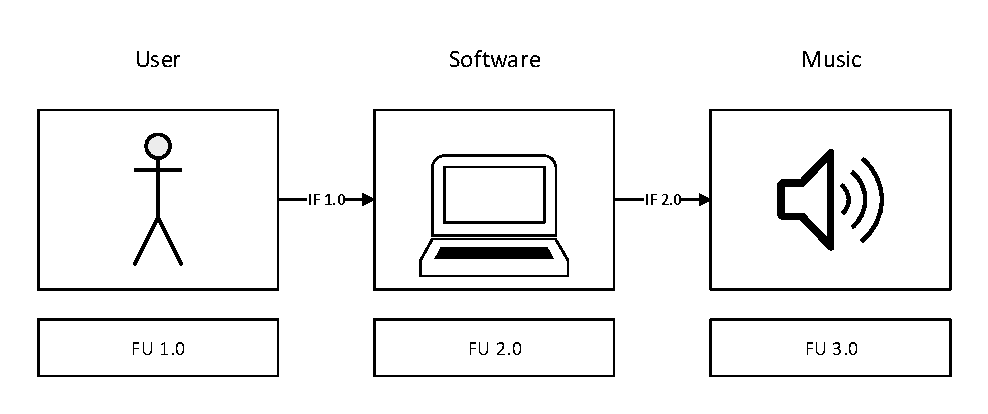
\includegraphics[width=300px]{../images/arch.pdf}}
\caption{Figure of high-level architecture of project}
\label{ims:archm}
\end{figure}

The solution to the problem is to create an application that is capable of composing and playing simple monophonic melodies using machine learning algorithms. Algorithms other than learning algorithms may be used, however these algorithms are narrow in application. Using learning algorithms and pattern recognition allows the application to produce melodies according to a selected style.

There is a need for a user-friendly application that can be used to generate simple monophonic melodies according to a certain style or category of music.
The application is required to have the following features:
\begin{enumerate}
\item Melodies are to be algorithmically composed according to a certain style.
\item Provide playback functionality as well as saving and loading of previously composed songs.
\item The user should be able to select the style.
\item The application should utilize a \acs{MIDI} library which will be used as training data for the machine learning algorithms.
\end{enumerate}

Figure \ref{ims:archm} indicates the interaction between the user and the software.

Since the quality and aesthetics of a musical melody is subjective, it is beyond the scope of the application to ensure that each melody produced is objectively good\footnote{The focus is rather on the generated musical pieces not being objectively bad}. Composed musical pieces will take the form of simple melodies.

\section{Alternative solutions}
A wide variety of research has been done and in this section we will briefly look at some of the existing solutions and their drawbacks.

\subsection{NEUROGEN}
NEUROGEN is a system that was designed to compose small diatonic, western-type, four-part harmony compositions based on a training set of example musical fragments. NEUROGEN tries to produce coherent music of the type that is typically found in traditionally hymns \cite{gibson1991neurogen}.
However NEUROGEN is only tries to fulfill its main research goals.

\subsection{CONCERT}
CONCERT incorporates psychologically-grounded representations of pitch, duration and harmonic structure in order to compose novel melodies. CONCERT uses a neural network in order to do note by note predictions. 

CONCERT struggles to compose natural music as the music produced was not globally coherent \cite{mozer1994neural}. 

CONCERT also only tries to fulfill its research goals, that is, to compose music on a note by note basis using a neural network.

More recent studies into recurrent neural networks based on \ac{LSTM} indicate that it is indeed possible to compose music using recurrent neural networks that have global structure \cite{Eck2002}.

\subsection{GenJam}
GenJam - Genetic Jammer is a \acs{IGA} that learns to improvise jazz \cite{Biles1994}.
The system is able to: 
\begin{enumerate}
\item Play full-chorus improvised solos
\item Respond interactively when the trumpet is played to trade fours or eights
\item Perform a smart echo of improvisation
\end{enumerate}

The main drawback of GenJam is that it is an interactive algorithm and as such requires input from the user. The creates a performance bottleneck as it is time-consuming for the user to rate musical pieces.
See section \ref{sec:iga} for work on \acsp{IGA}

\subsection{jMusic}
jMusic is an application and library that facilitates musical composition in Java \cite{Sorensen}. The application is designed to provide composers and developers a plethora of compositional tools that can be used for generative music, instrument building, interactive performance and music analysis. In addition the software provides the following:
\begin{itemize}
\item Familiar music data structures.
\item Organizing, manipulating and analyzing music data.
\item Real time playback of music scores.
\item Read, write \ac{MIDI}, \ac{XML} and .jm files.
\end{itemize}

jMusic is mostly a developer tool to facilitate composition. It does not feature a user interface which can be used to easily generate compositions. Furthermore since it is mostly a tool to aid music composition it does not employ machine learning algorithms. The library requires exact and descriptive input in order to generate melodies, and as such requires domain knowledge.

\subsection{Other}
Most of the work done in the field has been aimed at narrow application of the ideas being investigated. Thus algorithms and applications constructed were aimed only to experimentally study the ideas being investigated and not to serve as an end-user product. 

Some other small application exist which employ \acp{IGA} such as:
\begin{enumerate}
\item \href{http://askory.phratry.net/projects/evolutune/}{Evolutune}\footnote{http://askory.phratry.net/projects/evolutune/}
\item \href{http://www.compose-music.com/}{Song Builder}\footnote{http://www.compose-music.com/}
\item \href{http://game.darwintunes.org/}{DarwinTunes}\footnote{http://game.darwintunes.org/}
\end{enumerate}

Even though more recent research into algorithmic music composition yields promising results there is no single application combining the more recent research into a coherent application that is able to play monophonic melodies\footnote{In addition there is no accessible user-friendly application that expose machine learning based algorithmic composition to the user}.


\section{Feasibility}
There has been a plethora of research done into algorithmic music composition. Some of the more recent research that utilizes machine learning algorithms is investigated in chapter \ref{chap:comp_algo}.

Some machine learning methods to compose music algorithmically include:
\begin{itemize}
\item Recurrent neural networks \cite{Eck2002, mozer1994neural,Chen2001}
\item Genetic algorithms using \acs{NCD} as fitness functions \cite{Alfonseca2006,Dostal2013}
\item Genetic algorithms using neural networks as fitness functions \cite{gibson1991neurogen,Biles1996,Burton97geneticalgorithm}
\item Genetic algorithms employing Zipf's law and cosine similarity \cite{Dostal2013,Manaris2007,Manaris2005}
\item Interactive genetic algorithms \cite{Biles1994, Biles1996,Unehara,Spector_inductionand,Johanson1998}
\item Markov Chains for music composition \cite{McAlpine1999, Farbood2001}.
\item Hidden Markov Models for harmonization \cite{Allan2004}.
\item LSTM neural network for composing blues \cite{Eck2002}.
\end{itemize}

A variety of ideas and techniques in algorithmic music composition have already been researched. The difficulty arises in the implementation of the ideas (as the process is only fundamentally documented), representation of music in data structures and the implementation of the relevant machine learning algorithms.

\section{Methodology}
In Royce's classical waterfall model the following steps are followed when developing software:
\begin{itemize}
\item Requirements specification
\item Design resulting in the software architecture
\item Construction
\item Integration
\item Testing and debugging
\item Installation
\item Maintenance
\end{itemize}

Since there are a variety of algorithmic music composition strategies, and no formal analysis that compares the quality of the resulting music of each strategy (difficult as it is a subjective matter) the software prototyping methodology could be used to test these different ideas and to construct a trade-off study to determine the most feasible techniques.
\\
\\
Software prototyping is the development of prototypes - incomplete versions of the software.
Some basic principles of software prototyping include:
\begin{itemize}
\item Prototype selected parts
\item Breaking project into smaller segments
\item User or client may be involved
\item Iterative modification to meet user demands
\end{itemize}

The main ideas of the systems engineering process, as applicable to software will be followed. Ideas from the waterfall model and software prototyping will be incorporated.

The basic formulation of the design of the project is as follows:
\begin{enumerate}
\item Conceptual design
\begin{itemize}
\item Identify problem
\item Identify requirements
\item Resource allocation
\item Literature study
\item Feasibility analysis
\item Trade off study
\end{itemize}
\item Preliminary design
\item Detail design
\begin{itemize}
\item Design of software architecture
\item Prototyping of different strategies and algorithms
\end{itemize}
\item Construction
\begin{itemize}
\item Code is written
\item Code is tested
\item Iteratively improve until project meets specifications
\end{itemize}
\item Phase out, support, maintenance
\end{enumerate}

In order to identify suitable algorithms a literature review will be done. The various algorithms will be prototyped and tested and the best few resulting algorithms will be used. Software development will follow the waterfall model.

\pagebreak
\section{Conclusion}
Since the act of generating music using algorithmic means is of theoretical interest there is a plethora of research available, however most of these implementations only aim to explore the main idea being researched. Thus there is a lack of accessible, user-friendly applications that are able to generate music algorithmically.

The aim of this project is to construct an application that is able to compose music algorithmically. The application will utilize machine learning algorithms in order to compose monophonic melodies according to the style of a certain author or theme. These ideas have already been researched and thus the application is feasible. The only cost is time and effort.

The methodology for successfully completing the project is outlined and a schedule for completing each goal is presented. This should assist in meeting the deadlines and completing the project successfully according to the specifications. 